\section{Results}
\label{sec:results}
\subsection{Pretraining}
The evaluation loss curves during pretraining are displayed in \Cref{fig:eval-loss}. This figure shows that although no sparse models achieved lower evaluation loss than their respective baselines, at least one configuration from every sparse RoBERTa-based-models reached a similar loss as the baseline after one epoch, despite starting at a higher initial loss. Even among the GPT-Neo-based models, the MoE variant achieved a similar evaluation loss as the baseline.
\subsection{Evaluation}
\Cref{tab:summary_eval} demonstrates that all types of sparse feedforward layers can offer better performance for GPT-Neo and RoBERTa than FFN on (Super)GLUE tasks. As for BLiMP tasks, the PKM variant is unable to outperform the baseline for RoBERTa. The same applies to the MoE and PKM variants for GPT-Neo. On the other hand, the MoE variant performs consistently best on (Super)GLUE, while the CNT variant is the best on BLiMP. Detailed task scores for BLiMP and (Super)GLUE are reported by \Cref{tab:blimp} and \Cref{tab:superglue} in \Cref{appendix}.

\Cref{fig:spar-rat-super} and \Cref{fig:spar-rat} illustrate the relationship between the proportion of activate parameters (sparsity ratio) in the feedforward layer and the model performance on (Super)GLUE and BLiMP tasks respectively. The trend lines suggest that performance tends to increase with the sparsity ratio. However, this is not always the case, as the trend is reversed for RoBERTa-based models on (Super)GLUE tasks. Furthermore, the positive correlation between the sparsity ratio and performance is only moderate as indicated by the Pearson coefficients ($0.3 < r < 0.5$).
\subsection{Inference Speed}
\Cref{tab:inference} reports the average inference time per batch for each feedforward layer investigated. FFN is by far the fastest. This is followed by MoE, which is around $20\%$ slower. In comparison, CNT is more than twice as slow as MoE. PKM is much slower than all other kinds of feedforward layers.

\begin{figure}[!h]
    \centering
    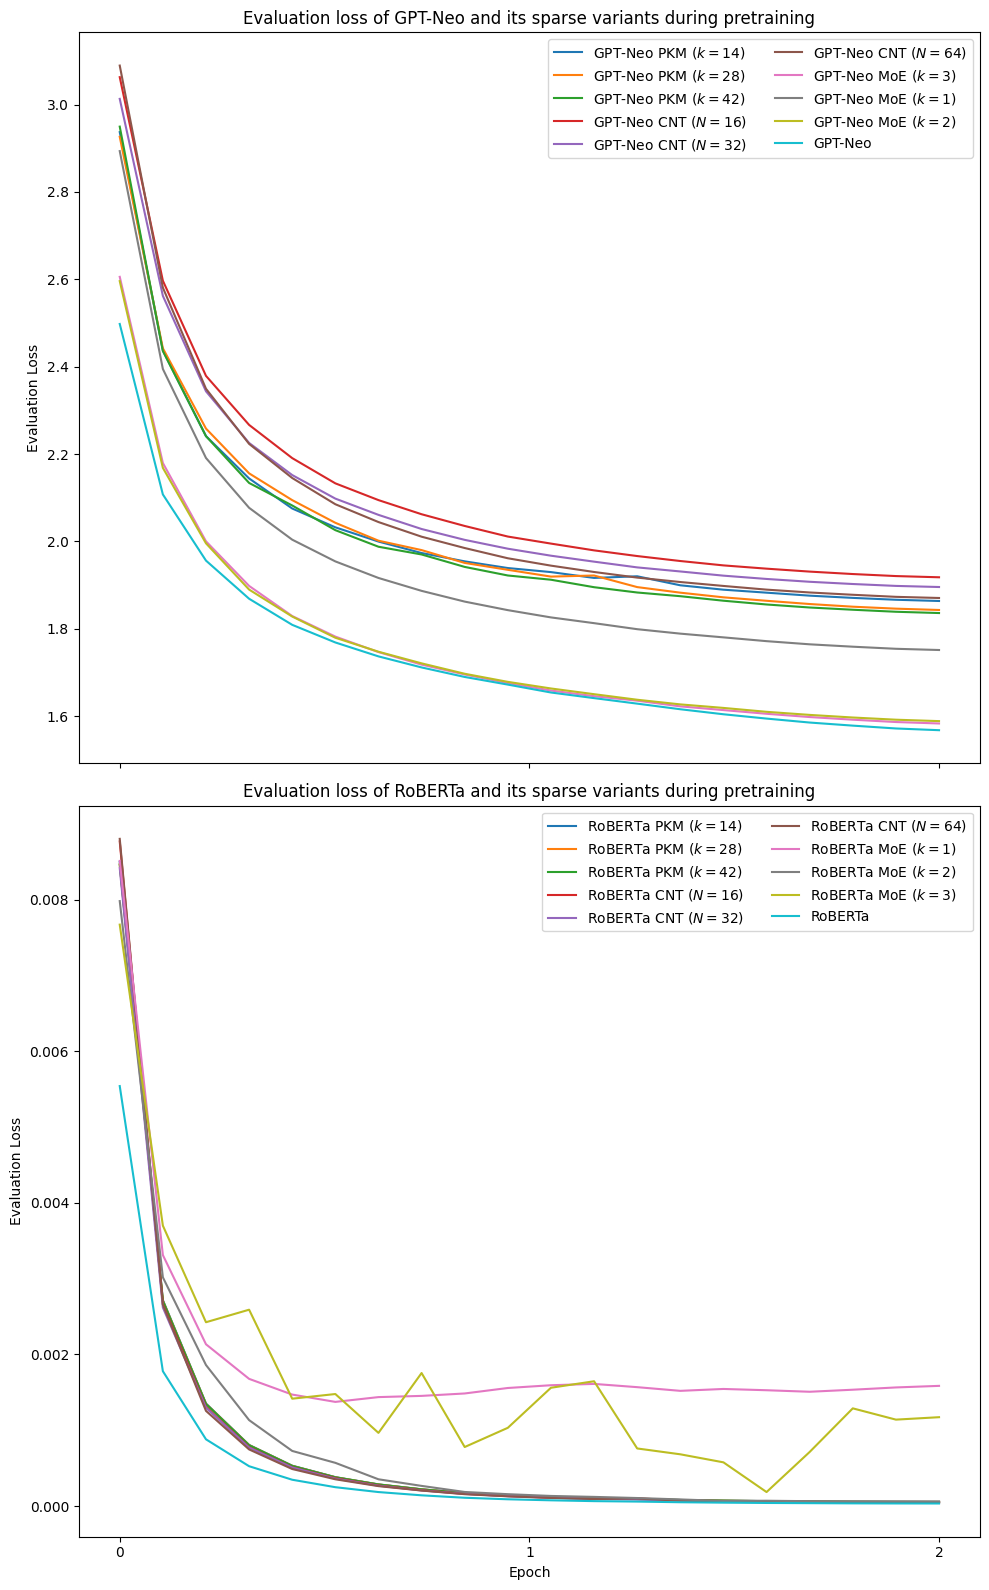
\includegraphics[width=0.5\textwidth]{evaluation_loss.png}
    \caption{Evaluation loss for GPT-Neo (top), RoBERTa (bottom), and their sparse variants during pretraining. Many sparse models reached a similar loss as the baseline by the end.}
    \label{fig:eval-loss}
\end{figure}

\begin{figure}[!h]
    \centering
    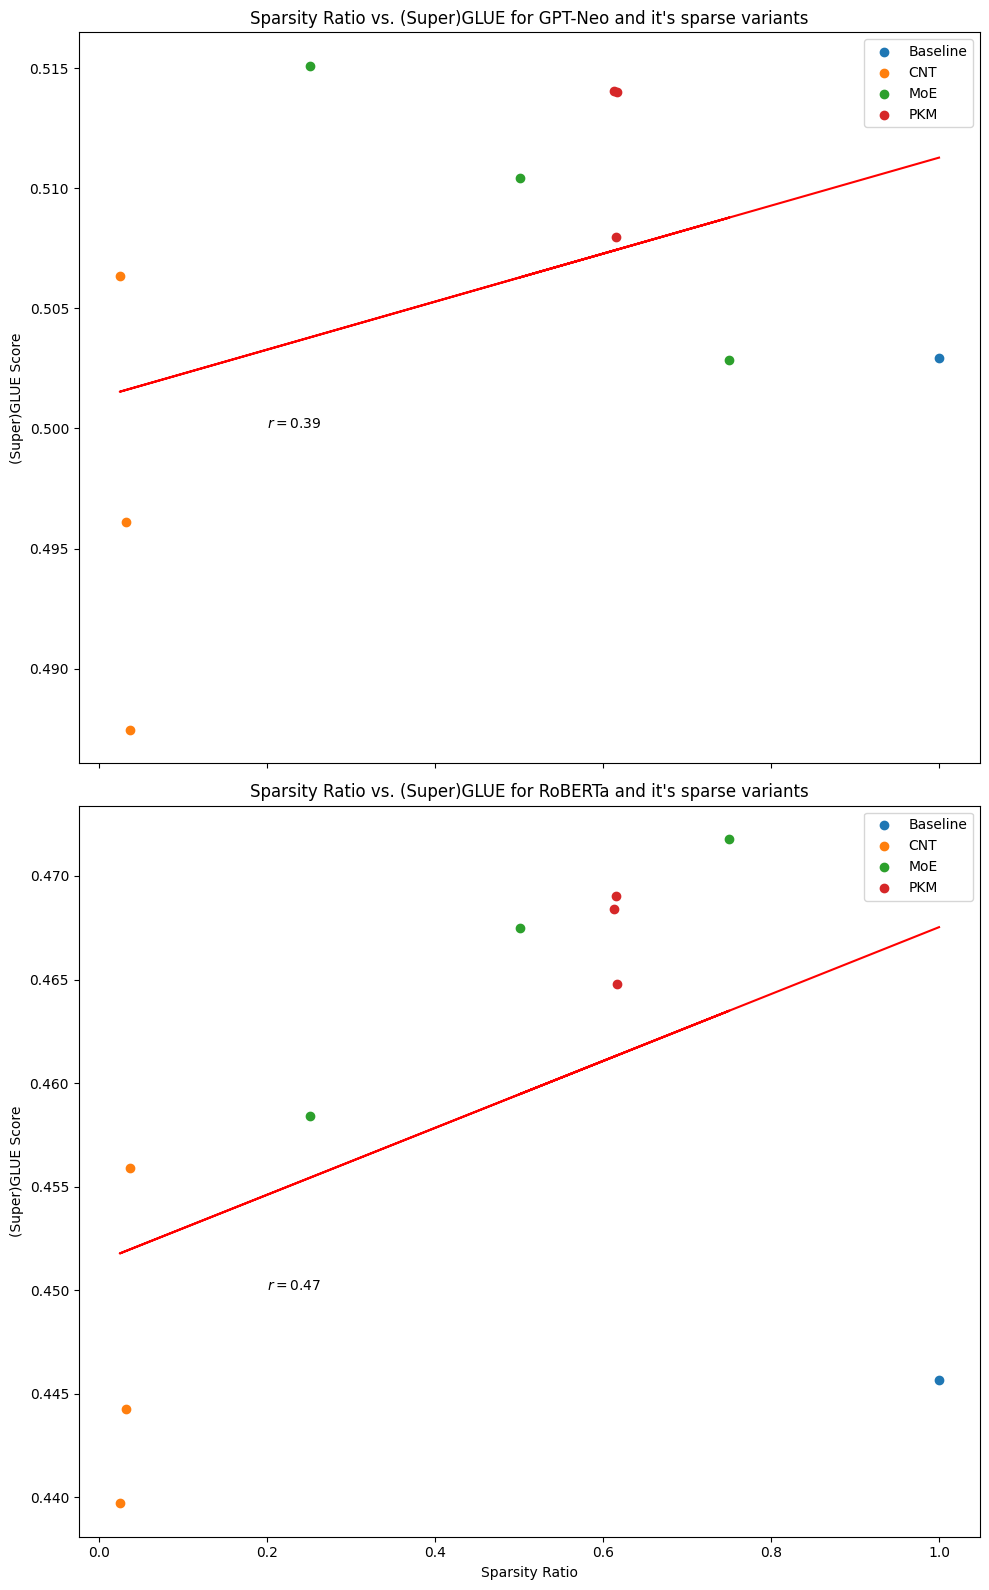
\includegraphics[width=0.5\textwidth]{sparsity_ratio_superglue.png}
    \caption{Sparsity ratio (percentage of active parameters in the feedforward layer) of the feedforward layers for GPT-Neo (top), RoBERTa (bottom) and their sparse variants vs. their respective overall (Super)GLUE scores. There is no strong correlation between the sparsity ratio and the (Super)GLUE score.}
    \label{fig:spar-rat-super}
\end{figure}

\begin{figure}[!h]
    \centering
    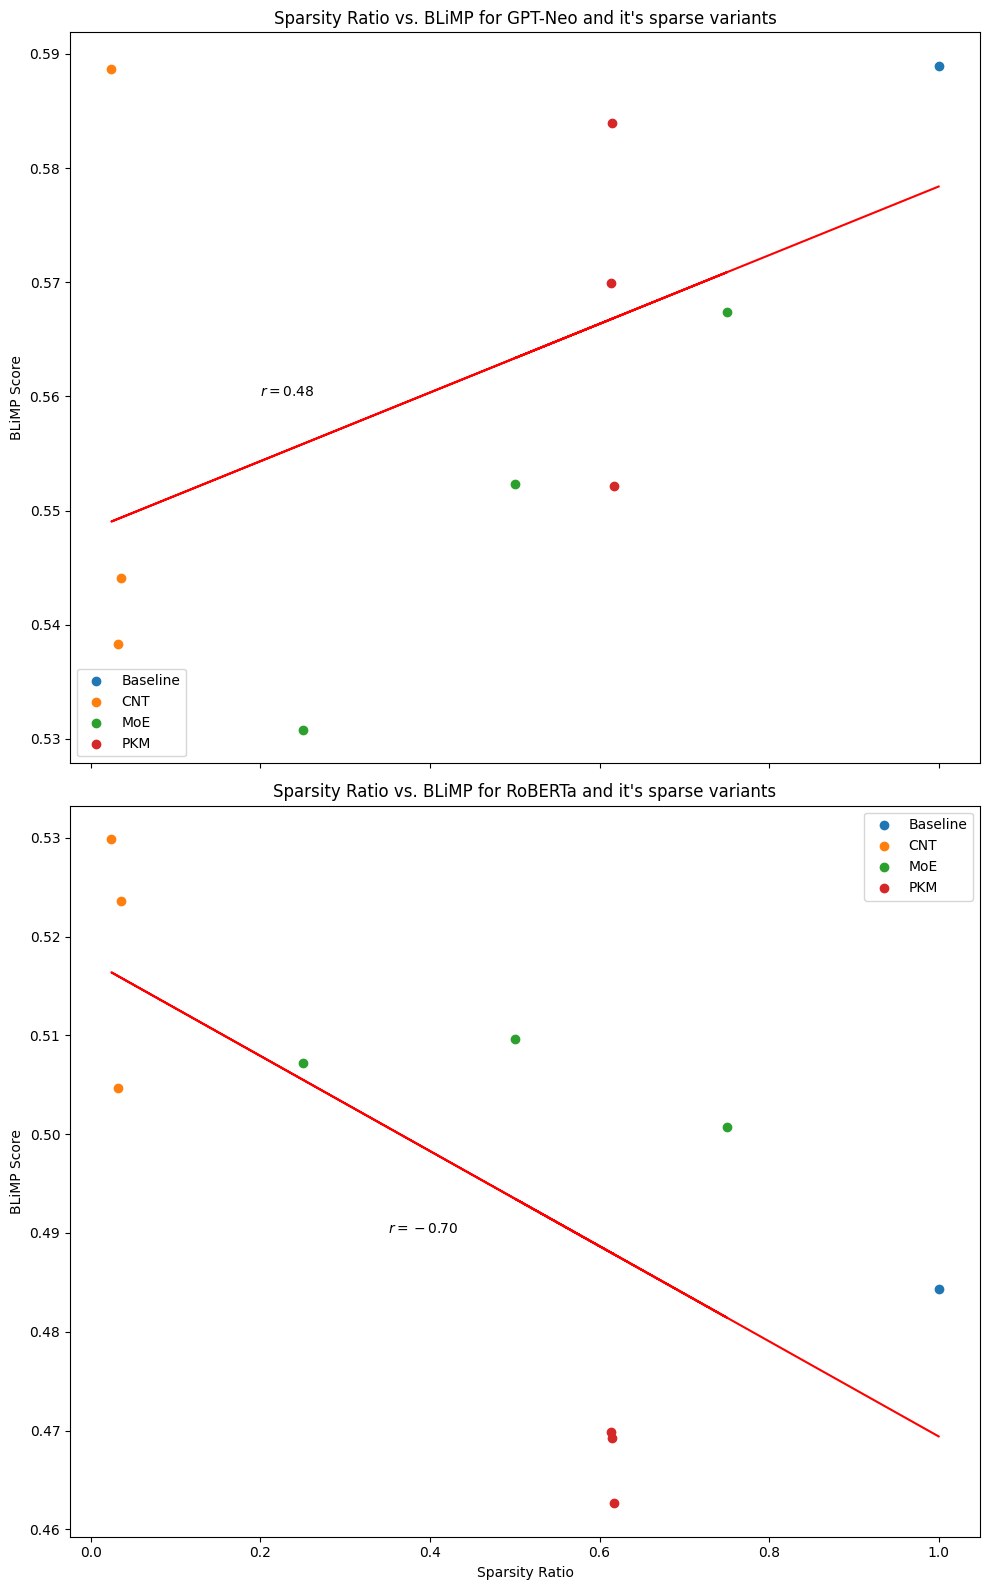
\includegraphics[width=0.5\textwidth]{sparsity_ratio.png}
    \caption{Sparsity ratio (percentage of active parameters in the feedforward layer) of the feedforward layers for GPT-Neo (top), RoBERTa (bottom) and their sparse variants vs. their respective overall BLiMP scores. There is no strong correlation between the sparsity ratio and the BLiMP score.}
    \label{fig:spar-rat}
\end{figure}

\begin{table}[h]
    \caption{BLiMP and (Super)GLUE scores for GPT-Neo, RoBERTa, and their sparse variants. The CNT variant is the best on BLiMP while the MoE variant is the best on (Super)GLUE.}
    \label{tab:summary_eval}
    \centering
    \tiny
    \begin{tabular}{lcc}
\toprule
Name & BLiMP & (Super)GLUE \\
\midrule
GPT-Neo & 0.589 & 0.503 \\
GPT-Neo CNT ($N=16$) & 0.544 & 0.487 \\
GPT-Neo CNT ($N=64$) & 0.538 & 0.496 \\
GPT-Neo CNT ($N=32$) & \textbf{0.589} & 0.506 \\
GPT-Neo MoE ($k=1$) & 0.531 & \textbf{0.515} \\
GPT-Neo MoE ($k=3$) & 0.567 & 0.503 \\
GPT-Neo MoE ($k=2$) & 0.552 & 0.510 \\
GPT-Neo PKM ($k=14$) & 0.570 & 0.514 \\
GPT-Neo PKM ($k=42$) & 0.552 & 0.514 \\
GPT-Neo PKM ($k=28$) & 0.584 & 0.508 \\
\hline
RoBERTa & 0.484 & 0.446 \\
RoBERTa CNT ($N=16$) & 0.524 & 0.456 \\
RoBERTa CNT ($N=64$) & 0.505 & 0.444 \\
RoBERTa CNT ($N=32$) & \textbf{0.530} & 0.440 \\
RoBERTa MoE ($k=1$) & 0.507 & 0.458 \\
RoBERTa MoE ($k=3$) & 0.501 & \textbf{0.472} \\
RoBERTa MoE ($k=2$) & 0.510 & 0.467 \\
RoBERTa PKM ($k=14$) & 0.470 & 0.468 \\
RoBERTa PKM ($k=42$) & 0.463 & 0.465 \\
RoBERTa PKM ($k=28$) & 0.469 & 0.469 \\
\bottomrule
\end{tabular}

\end{table}

\begin{table}[h]
    \caption{Batch inference speed of vanilla and sparse feedforward networks measured in milliseconds. FFN is faster than the sparse feedforward layers.}
    \label{tab:inference}
    \centering
    \begin{tabular}{lcc}
\toprule
Model & Mean (ms) & Standard Deviation (ms) \\
\midrule
Baseline & \textbf{12.83} & 0.10 \\
MoE ($k=1$) & 16.14 & 0.07 \\
MoE ($k=2$) & 16.24 & 0.08 \\
MoE ($k=3$) & 16.45 & 0.17 \\
CNT ($N=16$) & 34.42 & 0.09 \\
CNT ($N=32$) & 33.92 & 0.09 \\
CNT ($N=64$) & 34.06 & 0.25 \\
PKM ($k=14$) & 43.79 & 1.30 \\
PKM ($k=28$) & 77.35 & 3.00 \\
PKM ($k=42$) & 117.48 & 0.04 \\
\bottomrule
\end{tabular}
\end{table}